\documentclass[12pt, a4paper, twoside]{article}

%% Preamble
\usepackage{umatfgspanish}
\usepackage{blindtext}
\graphicspath{ {./images/} }

\begin{document}

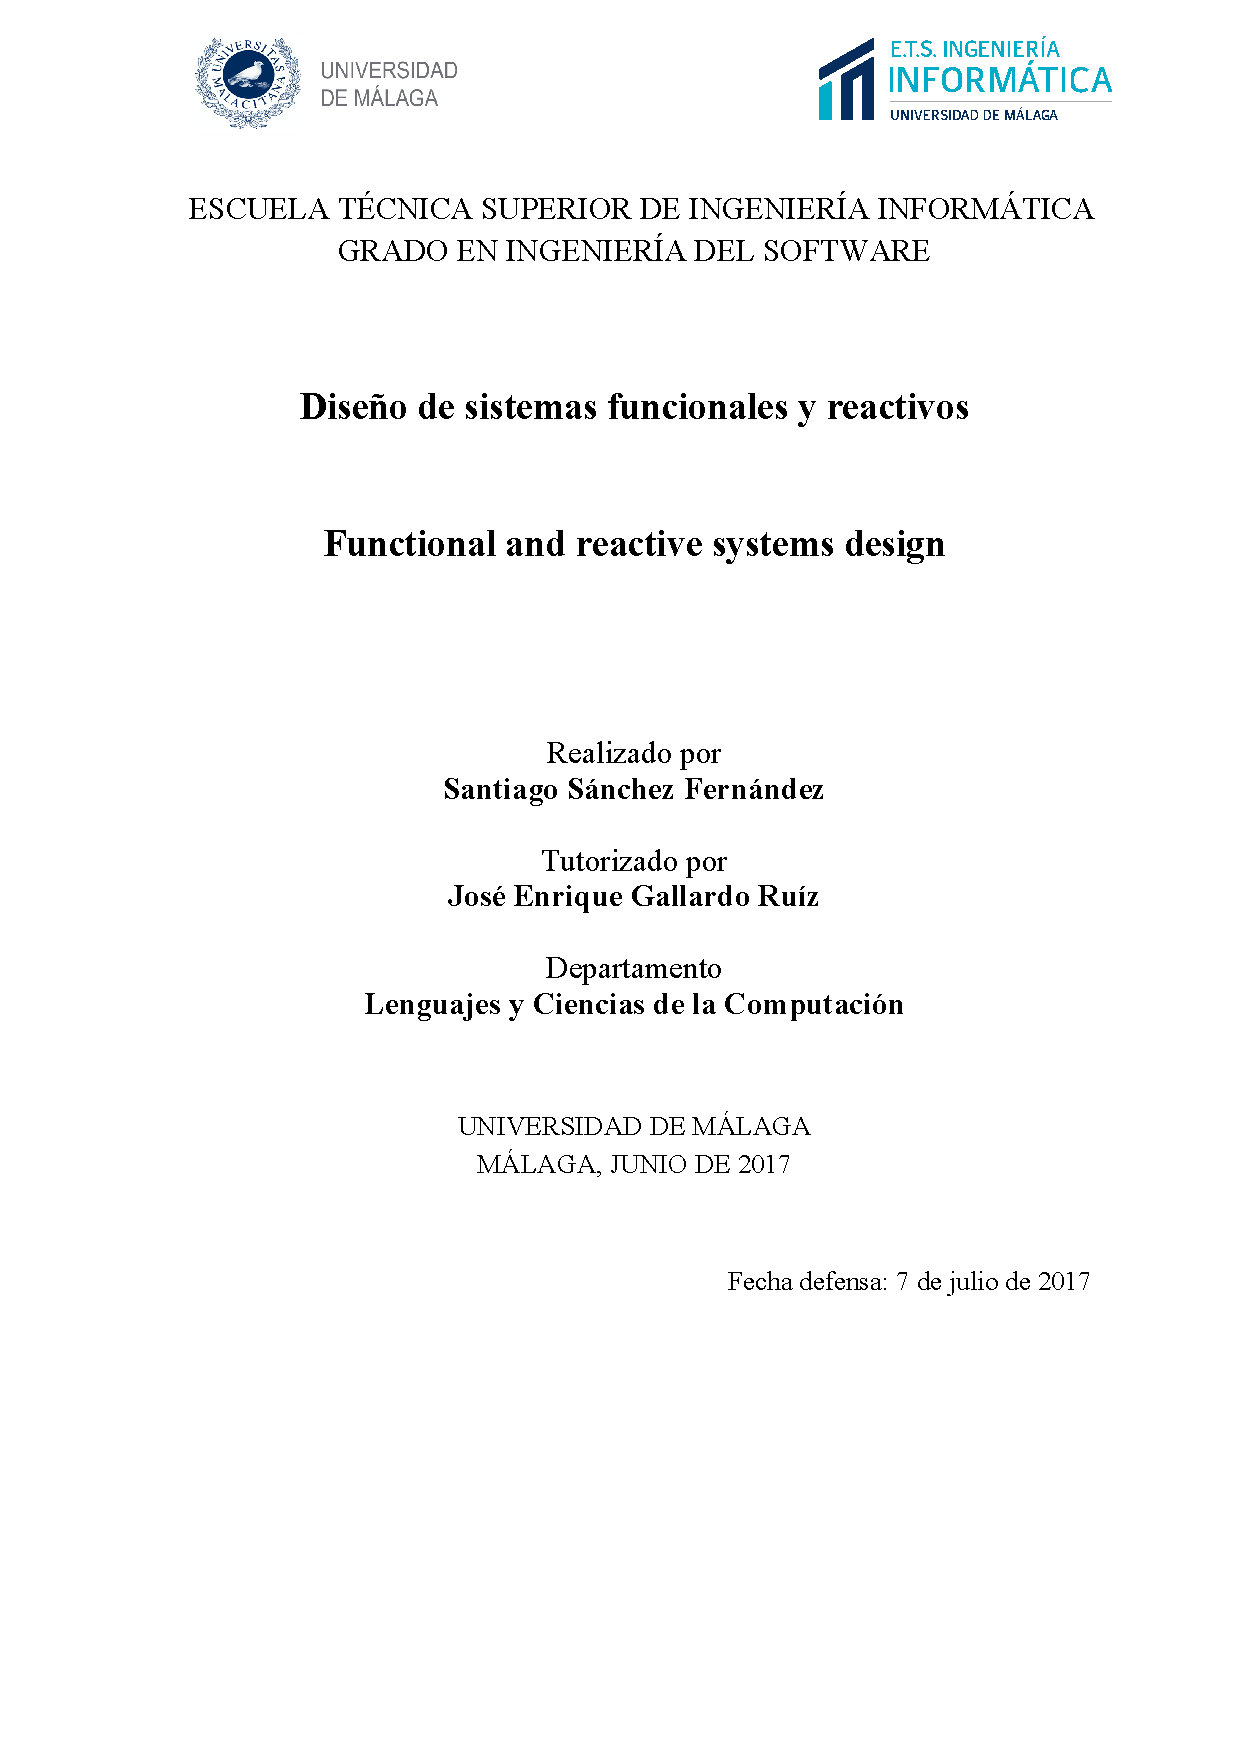
\includepdf[noautoscale=true, width=\paperwidth]{title.pdf}

\newpage

%% Abstract
\begin{abstract}

  \subsection{Español}
    Iot es una red de objetos físicos que están incrustados con electrónica, software, 
sensores y conectividad de red, lo que permite a estos objetos recopilar y intercambiar datos.
 La IoT permite que los objetos sean detectados y controlados de forma remota a través de la 
 infraestructura de red existente, creando oportunidades para una integración más directa del mundo 
 físico en los sistemas basados en computadora, y resultando en una mayor eficiencia, precisión y 
 beneficio económico además de una reducción de la intervención humana.

\subsection{English}
IoT is a network of physical objects that are embedded with electronics, 
software, sensors, and network connectivity, which enables these objects 
to collect and exchange data. The IoT allows objects to be sensed and controlled 
remotely across existing network infrastructure, creating opportunities for more 
direct integration of the physical world into computer-based systems, and resulting 
in improved efficiency, accuracy and economic benefit in addition to reduced human 
intervention.

	\bfseries{\large{Keywords:}} IoT, FIWARE, Edificios Inteligentes
\end{abstract}

\tableofcontents

%% Sections
\section{Introducción \\}
Introducción (incluyendo la motivación y objetivos del TFG, así como la estructura del resto de capítulos de la memoria).
\subsection{Motivation}
De acuerdo con (Estevez et al., 2021), la densidad de población que habita en las ciudades crece aceleradamente.
Se espera que para el 2030, un 60\% de las personas viva en las ciudades. 

Al existir una migración tan importante de áreas rurales a urbanas, el entorno de la
propia ciudad evoluciona más rápido y los retos a los que estas se enfrentan, o se espera que se enfrenten,
también cambian notablemente: el transporte, impacto medioambiental, salud pública, servicios, etc. Son puntos
críticos que merecen especial atención para mantener y mejorar el funcionamiento y la calidad de vida en
las urbes.

Todo esto, junto al crecimiento de las infraestructuras de telecomuncación (Banda ancha, wifi y 5G)
y a las inversiones en inteligencia artificial y big data, convierten  a Internet de las cosas (IoT)
 en un posible candidato para implementar soluciones y ofrecer mejoras a los gobiernos y ciudadanos, 
que ayuden a mejorar la gestión de las ciudades, la calidad de vida en las mismas y 
sean lo más respetuosas posible con el entorno.

Desde que se empezó a hacer uso del concepto de IoT, se puede ver que ha tenido una evolución favorable
 y ha mejorado en muchos aspectos,
de hecho, según (
    Elnashar, A. \& El-saidny, M. (2018). IoT evolution towards a super-connected world. Wiley. \textit{Practical Guide to LTE-A, VoLTE and IoT: Paving the way towards 5G}. pp. 310-381. Wiley. https://doi.org/10.1002/9781119063407.ch7
  Ayman Elnashar; Mohamed A. El-saidny, "IoT Evolution Towards a Super‐connected World," in Practical Guide to LTE-A, VoLTE and IoT: Paving the way towards 5G , Wiley, 2018, pp.310-381, doi: 10.1002/9781119063407.ch7.
  , En los últimos años, el uso del IoT ha aumentado exponencialmente,
  )
  el presupuesto invertido en la IoT ha incrementado, el número de dispositivos ha crecido
exponencialmente, ...

Es destacable mencionar que la situación global de la COVID-19 ha incentivado y acelerado la aplicación
de la IoT en diversos aspectos como la salud pública, la seguridad o la privacidad.

    \begin{figure}[h]
      \centering
        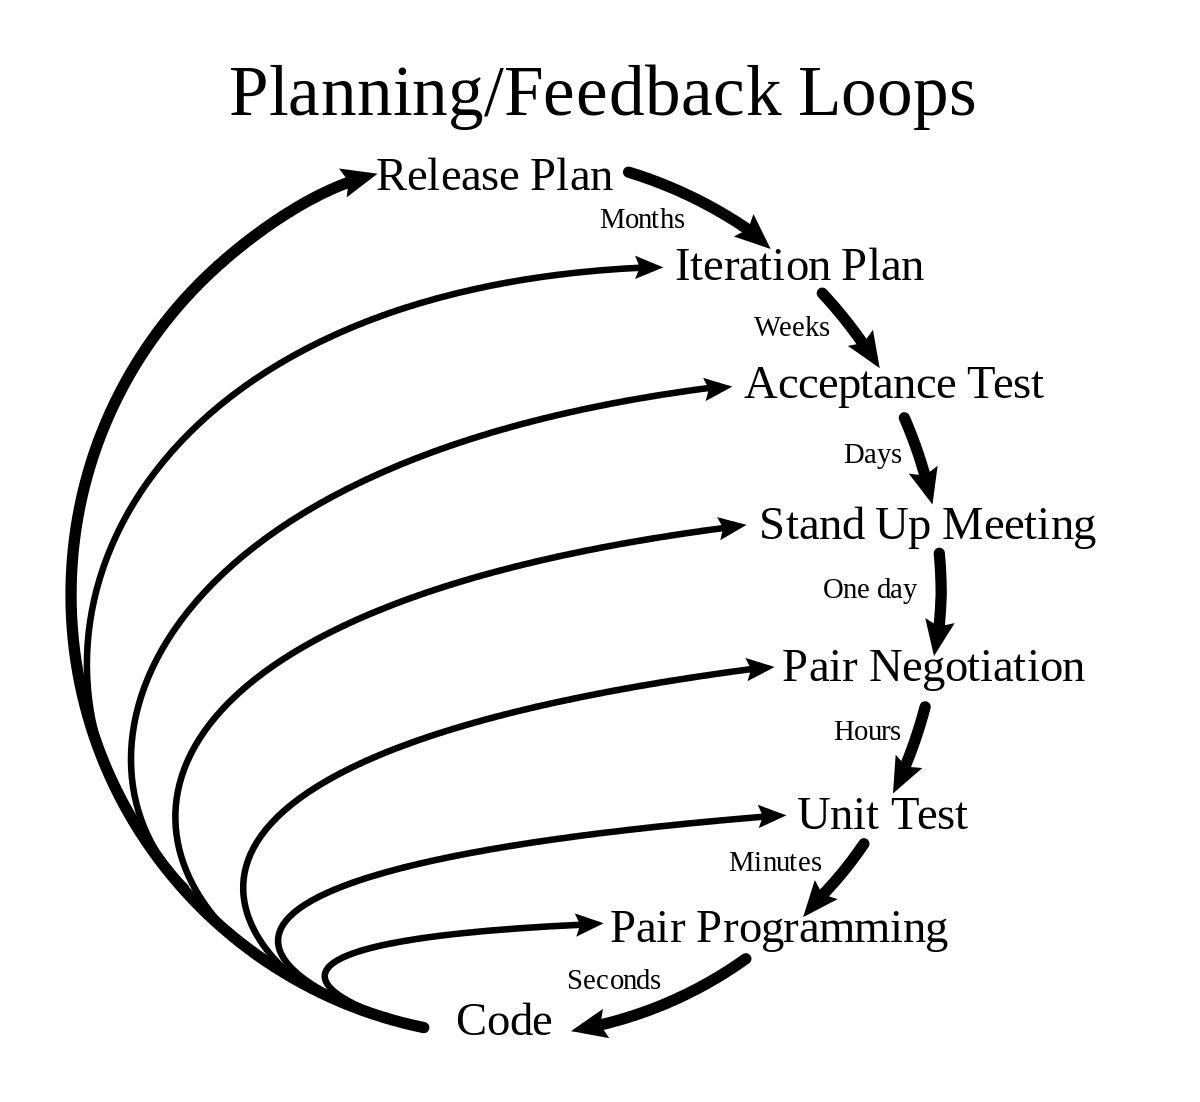
\includegraphics[width=0.5\textwidth]{xp}
      \caption{A diagram showing the iterations of extreme programming.}
    \end{figure}
    
    \blindtext[4]
\subsection{Objetivos}
El objetivo será desarrollar un sistema que, usando IoT, genere un digital twin de un Edificio
\subsection{Estructura del documento}

\section{Estudio del arte \\}
En esta sección se va a realizar un análisis de las tecnologías que se van a emplear para el 
desarrollo del Software. Para ello, se va a comenzar con una revisión exahustiva del IoT: 
Qué es, qué podemos hacer con esta tecnología y qué problemas presenta que se deban de tener en cuenta,
 para tener un punto de partida a la hora de elegir las tecnologías a utilizar.
 \subsection{Internet de las Cosas}
 Internet consiste en una red de usuarios y servidores conectadas entre sí.
 Sin embargo, existen conceptos más amplios que abarcan un conjunto de elementos todavía más ambicioso,
 como es el de Internet de las cosas (IoT), que, además de los anteriores, incluye a cualquier 
 objeto físico como participante de la red: IoT es una red de objetos físicos que están incrustados 
 con electrónica, software, sensores y poseen conectividad a la red, lo que permite a estos objetos
 recopilar y intercambiar datos. IoT permite que los objetos sean detectados y controlados de forma 
 remota a través de la  infraestructura de red existente, creando oportunidades para una integración 
 más directa del mundo físico en los sistemas basados en computadora, y resultando en una mayor 
 eficiencia, precisión y beneficio económico además de una reducción de la intervención humana. 
 
 De esta forma podemos ser capaces de interactuar con los objetos de manera remota, sin intervención física de
 una persona, o de manera automática.
 
 Además, podrían realizar sus tareas de forma más inteligente, ya que, al estar conectadas a internet, pueden
 disponer de mucha información útil para su objetivo.

Sumado a lo anterior, IoT es una tecnología relativamente reciente y son muchos los campos en los que 
todavía se puede aplicar para sacar ventaja. El potencial es muy elevado, y eso se puede ver en
conceptos como:
\begin{itemize}
  \item \textbf{IoT Orchestation}, que permite organizar los dispositivos para combinar sus operaciones
  y resultados, concediendo al sistema un mayor nivel de inteligencia.
  \item \textbf{Fog Computing}, que permite optimizar la comunicación entre dispositivos, evitando llamadas
  innecesarias a los servidores, mejorando la eficiencia y sostenibilidad.
  \item \textbf{Digital Twin}, que se trata de un modelo que representa digitalmente lo mas fiel posible
   un sistema real, con el cual consultar su estado de una manera sencilla y simular supuestos
   (SandBbox) para observar qué pasaría y como afecta al sistema en general.
\end{itemize}
Todas esta características pueden aportar para una transformación digital inteligente y sostenible de las ciudades.

Entre de las ventajas más destacadas a la hora de usar IoT, podemos mencionar:
\begin{itemize}
    \item La sensorización: Permite obtener datos que anteriormente no podían ser recogidos de manera automática.
    \item Acciones remotas: Los objetos que se conectan a la red pueden realizar acciones físicas desencadenadas por internet,
      por lo que no tiene haber nadie presente ante el objeto para poder manipularlo o monitorizar su estado.
    \item Interacción entre dispositivos IoT: Gracias a los modelos de comunicación, se pueden realizar tareas complejas
      comunicando diferentes sensores y actuadores, de esta forma, se producen una secuencia de acciones sin necesidad
      de intervención humana, que produce unos resultados dignos de categorizar como inteligentes.
\end{itemize}


Por otro lado, al analizar el avance del IoT desde sus comienzos, se puede llegar a la conclusión 
de que ha ocurrido muy rápido, y todavía hay muchos puntos en los que debe de madurar:
 - Interfaces de Estandarización (Discovery, semántica de datos)
 - Data Swamp (Discovery)

 Por lo que a la hora de hacer un desarrollo usando IoT se deben de tener en cuenta estos aspectos.


 Según el punto de vista de Fiware, las ciudades tienen 5 etapas en su camino a la digitalización inteligente:
 - 
 -
 -
 -
 -



  \subsection{Plataforma FIWARE} 
 Para el desarrollo de la plataforma, se ha decidido utilizar FIWARE.
 
Esta plataforma consisten en un conjunto de componentes de software que permiten la creación 
de aplicaciones basadas en la nube, por ejemplo se pueden utilizar para crear aplicaciones de 
Internet de las cosas (IoT). 

FIWARE se basa en la arquitectura de software de código abierto, que se puede utilizar para crear 
aplicaciones de IoT y aplicaciones de IoT inteligentes.

  \subsection{Ontología SAREF}
  Se trata de una interfaz de datos que le gusta la UE.

  Gracias a ngsi-ld, podemos hace uso del modelo de datos.

 \section{Metodología de trabajo}
 Metodología de trabajo empleada en el TFG (esta parte también puede incluirse como una sección del capítulo de Introducción o como un capítulo independiente).

 \section{Fases del proyecto (se procede)}
 Capítulos donde se estructure las fases del desarrollo, así como pruebas y resultados (si procede). 

\section{Conclusións e liñas de traballo futuras}
Conclusiones y Líneas Futuras. En caso de redactarse la memoria en inglés, las conclusiones y líneas futuras deben redactarse también en castellano.

\section{Contraportada}
%% Bibliography
\begin{thebibliography}{9}
  \bibitem{Awa}
  Estevez E., Pardo, T., \& Scholl, J. (2021).
Smart cities and smart governance: towards the 22nd century sustainable city. Springer.
    \textit{The \LaTeX\ Companion}. 
    Addison-Wesley, Reading, Massachusetts, 1993.
    
    \bibitem{einstein} 
    Albert Einstein. 
    \textit{Zur Elektrodynamik bewegter K{\"o}rper}. (German) 
    [\textit{On the electrodynamics of moving bodies}]. 
    Annalen der Physik, 322(10):891–921, 1905.

\end{thebibliography}

\newpage

%% Apendices
\begin{umaappendices}
\section{Installation \\ Manual}
Apéndices: información complementaria que no tenga cabida en el cuerpo del TFG, tales como listados, descripciones detalladas, manuales de usuario y programador, etc. 
    
    \textbf{\large{Requirements:}}
    
    \blindtext

\end{umaappendices}

\end{document}
